\documentclass[11pt,oneside,english,a4paper]{article}

\usepackage{a4wide}
\usepackage[T1]{fontenc}
\usepackage{amsmath}
\usepackage{pxfonts}
\usepackage[latin1]{inputenc}
\usepackage{longtable}
\usepackage[pdftex]{hyperref}
\hypersetup{colorlinks=true,urlcolor=blue}

%\usepackage{textcomp}   % Give the degree symbol using \textcelsius
%\usepackage{epsfig}



%\usepackage{natbib}
%\usepackage{verbatim}
\usepackage[pdftex]{color,graphicx}

\setcounter{secnumdepth}{10}

\pagestyle{headings}

\setlength{\baselineskip}{2.0\baselineskip}
\renewcommand{\thesection}{\arabic{section}}

\newcommand{\InsFig}[4]{%
	\begin{figure}[!htb]%
	\begin{center}%
	\includegraphics[width=#2\linewidth]{#1}%
	\end{center}%
	\caption{#3\label{#4}}%
	\end{figure}}


\begin{document}
\title{ePic2 Documentation}
\author{Julien Hubert}
%\date{}
\maketitle
\section{Introduction}
The ePic2 software is a toolbox to interface Matlab with an e-puck(for additional information see \href{http://www.e-puck.org}{http://www.e-puck.org}). It contains a graphical interface and a set of primitives allowing to send and receive commands between the e-puck and Matlab. It will be used in the laboratories of the course Robots Mobiles (\href{http://moodle.epfl.ch/course/view.php?id=261}{http://moodle.epfl.ch/course/view.php?id=261}). The goal of the software is to provide students with the necessary tools to explore the topic of mobile robotics while focusing on high level behaviors or strategies.
\par The next section will present the commands to interact with the e-puck available from the Matlab command line. Following, the graphical interface and its possibilities will be described.

\section{Quickstart}
This section intends to give you the quick steps needed to start working with ePic2.
\begin{enumerate}
\item \textbf{epic=ePicKernel;} creates a class containing all the variables needed to command the e-puck
\item \textbf{epic=connect(epic,'COMXX');} will connect epic to an e-puck accessible through the serial port COMXX
\item \textbf{epic=update(epic);} updates the status of the physical e-puck and of the epic class. It transfers data from and to the e-puck. 
\item \textbf{epic=disconnect(epic);} breaks the connection between the e-puck and Matlab.

\end{enumerate}

\section{Matlab Commands}
\subsection{The ePicKernel class}
ePic2 is based on a class containing all the information related to the e-puck. This class contains the values of the sensors, their rate of update, the commands that should be sent to the e-puck and the inner parameters of the ePic2 interface.
\par To act on the e-puck, the class contains a set of functions setting some inner variable related to its control. Those will be detailed in the following sections.
\par The class is created by calling \emph{epic=ePicKernel;}.

\subsection{Connection to the E-Puck}
Before sending commands to the e-puck, the function \emph{connect} must be called. This function takes as parameters an instantiation of the class ePicKernel and a string containing the COM port associated with the e-puck. For instance,  \emph{epic=connect(epic,'COM15')} opens a connection with the e-puck associated to port COM 15. The command returns a modified instance of the ePicKernel class. If the connection was successful, the command \emph{get(epic,'connectionStatus')} returns 1, otherwise 0.
\par Once connected, all the interactions will be done with the same robot. It is not possible to connect to more than one e-puck at a time due to Matlab limitations.
\par To disconnect, the command \emph{epic=disconnect(epic)} should be called. Afterward, Matlab can be connected to another e-puck on another port.

\subsection{Sending and Receiving Data}
All the interactions with the e-puck, with the exception of the camera, are centralized in one command \emph{epic=update(epic);}. This command updates the values of the sensors and sends the commands to the e-puck. 
\par All the transfers between the e-puck and Matlab are done simultaneously. First, all the commands are sent to the e-puck. Those can be a request for sensor values or a modification of the e-puck's wheel speed. Then, \emph{update} waits for the reception of the requested information and updates the variables of the class epic.
\par It is also possible to send custom commands to the e-puck using the low level functions to send and receive data. Those exist either in ASCII or in binary but their usage is the same. The difference resides in the way the data are encoded. In ASCII mode, the data sent by the e-puck are formatted as a string. The Matlab command \emph{str2num} has to be called to convert those into a Matlab variable. In binary mode, the data are formatted as they were on the e-puck and spread over different bytes. It is then necessary to reformat the values into their original format. This is generally more difficult to do as it requires a knowledge of the inner programming of the e-puck. The binary mode is nevertheless more advantageous when multiple commands have to be sent simultaneously. In ASCII mode, all commands are sent separately on the bluetooth channel while in binary the are all sent with one transfer only. This has the effect of speeding up the transfers between the e-puck and Matlab.
\par Sending a custom command is done through the functions \emph{write(epic,data);} or \newline \emph{writeBin(epic,data);} where data contains the commands to send. The first function uses the ASCII mode while the second the binary mode. Those commands are asynchronous and won't wait for the answer of the e-puck. To receive the result of the sent command, the functions \emph{data=read(epic);} or \emph{data=readBin(epic);} have to be called according to the type of writing you did previously. An alternate command to read binary data is \emph{data=readBinSized(epic,n);} where \emph{n} is the size in bytes of the data to be transfered. The function will wait until all the data has been received or for a timeout to occur.
\par The final command to know is \emph{flush(epic);} which resets the transmission and reception buffer of Matlab. It is useful to call before any communication with the e-puck as Matlab does not seem to do it by itself. If not called, there are risks that old information will remain in the buffers.

\subsection{Commanding the e-puck}
As mentioned earlier, the \emph{update} command handles all the information transfers between Matlab and the e-puck. All data sent or received is stored in the class' variables. By default, ePic2 reads the values of the accelerometer, the proximity sensors, the light sensors, the microphones, the motor speeds and the encoders. Those correspond to the basic functionalities of the e-puck.
\par To activate the reading of a sensor, the command \emph{epic=activate(epic, propName, frequency);} must be called where \emph{propName} is the name of the sensor to activate and \emph{frequency} if it must be read always or only once at the next \emph{update}. To deactivate a sensor, the command \emph{epic=deactivate(epic, propName);} must be used.
\par Once the information has been retrieved, it can be obtained with the function \newline \emph{[val,up]=get(epic,propName);} where \emph{val} contains the requested values and \emph{up} indicates those were refreshed during the last update.
\par The following table contains the values for \emph{propName} and should be used as Matlab strings.
\setlongtables
\begin{longtable}{|l|l|p{4.8cm}|}
\hline
propName & Data & Supported Commands\\
\hline
accel & Accelerometers & get, activate, deactivate\\
\hline
proxi & Proximity Sensors & get, activate, deactivate\\
\hline
light & Light Sensors & get, activate, deactivate\\
\hline
micro & Microphones & get, activate, deactivate\\
\hline
speed & Motor Speeds & get, activate, deactivate\\
\hline
pos & Encoders & get, activate, deactivate\\
\hline
odom & Odometry Position & get, activate, deactivate\\
\hline
external & LIS External Sensor Turret & get, activate, deactivate\\
\hline
image & Camera Image & get, activate, deactivate\\
\hline
custom & Custom Command & get, activate, deactivate\\
\hline
connectionState & Connection Status & get\\
\hline
\end{longtable}

\par The command \emph{epic=set(epic,varargin);} modifies some properties of the e-puck. \emph{varargin} is a set of parameters beginning with the name of the property to modify followed by a vector containing the new values. For instance, to set the speed of the two motors, the command \emph{epic=set(epic,'speed',[100 100]);} must be called. The following table details the supported properties and their arguments.
\setlongtables
\begin{longtable}{|l|l|p{4.8cm}|}
\hline
propName & Arguments & Description\\
\hline
speed & [right\_motor left\_motor] & Change the motor speeds\\
\hline
ledOn & [led\_number] & Light on the led number led\_number\\
\hline
ledOff & [led\_number] & Light off the led number led\_number\\
\hline
odom & [x y theta] & Set the current position used by the odometry\\
\hline
camMode & [mode] & Set the camera mode (0: grayscale, 1:color)\\
\hline
camSize & [width height] & Set the width and the height of the camera\\
\hline
camZoom & [zoom] & Set the zoom factor (1, 4 or 8)\\
\hline
external & [options] & Select the external sensor and set its options\\
\hline
ledIR & [leds] & Set the leds to light on or off for the 5 leds external sensor\\
\hline
custom & [commands, amount of bytes to receive] & Set a custom command to be executed by the e-puck\\
\hline
\end{longtable}

\par The \emph{update} function cannot get an image from the camera of the e-puck. This is due to the long time needed to transfer the image from the robot to the computer and also to the specific processing done on it. To request an image, the command \emph{[epic, mode, sizexy]=updateImage(epic);} must be called. The returned values mode and sizexy are respectively the color mode of the camera and the size of the image. Once done, use the command \emph{[image,up]=get(epic,'image');} to retrieve the stored image from the class.

\par ePic2 can compute the odometry of the robot. For that purpose, the function \newline \emph{[epic]=updateOdometry(epic);}. As before, the function \emph{[pos,up]=get(epic,'odom');} returns the position of the robot. The function \emph{epic=reset(epic,'odom');} will reset the internal variables of the odometry. The command \emph{set} can also modify those variables. More details concerning its use have been given above.

\par ePic2 supports the use of custom commands. A custom command is a vector containing Sercom instructions that will be sent to the e-puck during the next update. They will be executed at the end of the regular commands. The results can be retrieved with \emph{get(epic,'custom')}. Those will be raw data in a 8 bits format. It can be necessary to convert them to Matlab's format. Many examples of this can be found in the source code of the \emph{update} function and a function \emph{two\_complement} receiving two 8 bits values and returning their equivalent in 16 bits is provided with ePic2.

\subsection{The Filters}
It is sometimes interesting to apply some processing on the readings of a sensor. For instance, the calibration of the proximity sensors is necessary to use them. To allow this in a transparent way, some empty filters have already been created. The functions \emph{filter\_Accel, filter\_Light, filter\_Micro, filter\_Prox} and \emph{filter\_image2} are called every time a reading is done on respectively the accelerometer, the light sensors, the microphones, the proximity sensors and the camera. They receive as argument the data and return the filtered values of those. When no filter is implemented, the returned values are the same as the read values. In case of the need for a filter, those functions can be rewritten according to the user needs.

\section{The Graphical Interface}
The graphical interface has been developed to display the status of the e-puck in real-time. Its programming relies on the above mentioned commands but add some functionalities. The interface is refreshed on a regular interval and can show the values of the sensors in real time, it allows to command the movements of the robots using a joystick-like interface, it displays the camera snapshots before and after filtering and also plot the path of the robot using odometry. All those can be seen in figure \ref{fig:epic}.
\par The interface possesses a menu where sensor readings can be activated or deactivated.

\begin{figure}[htb]
	\centering
		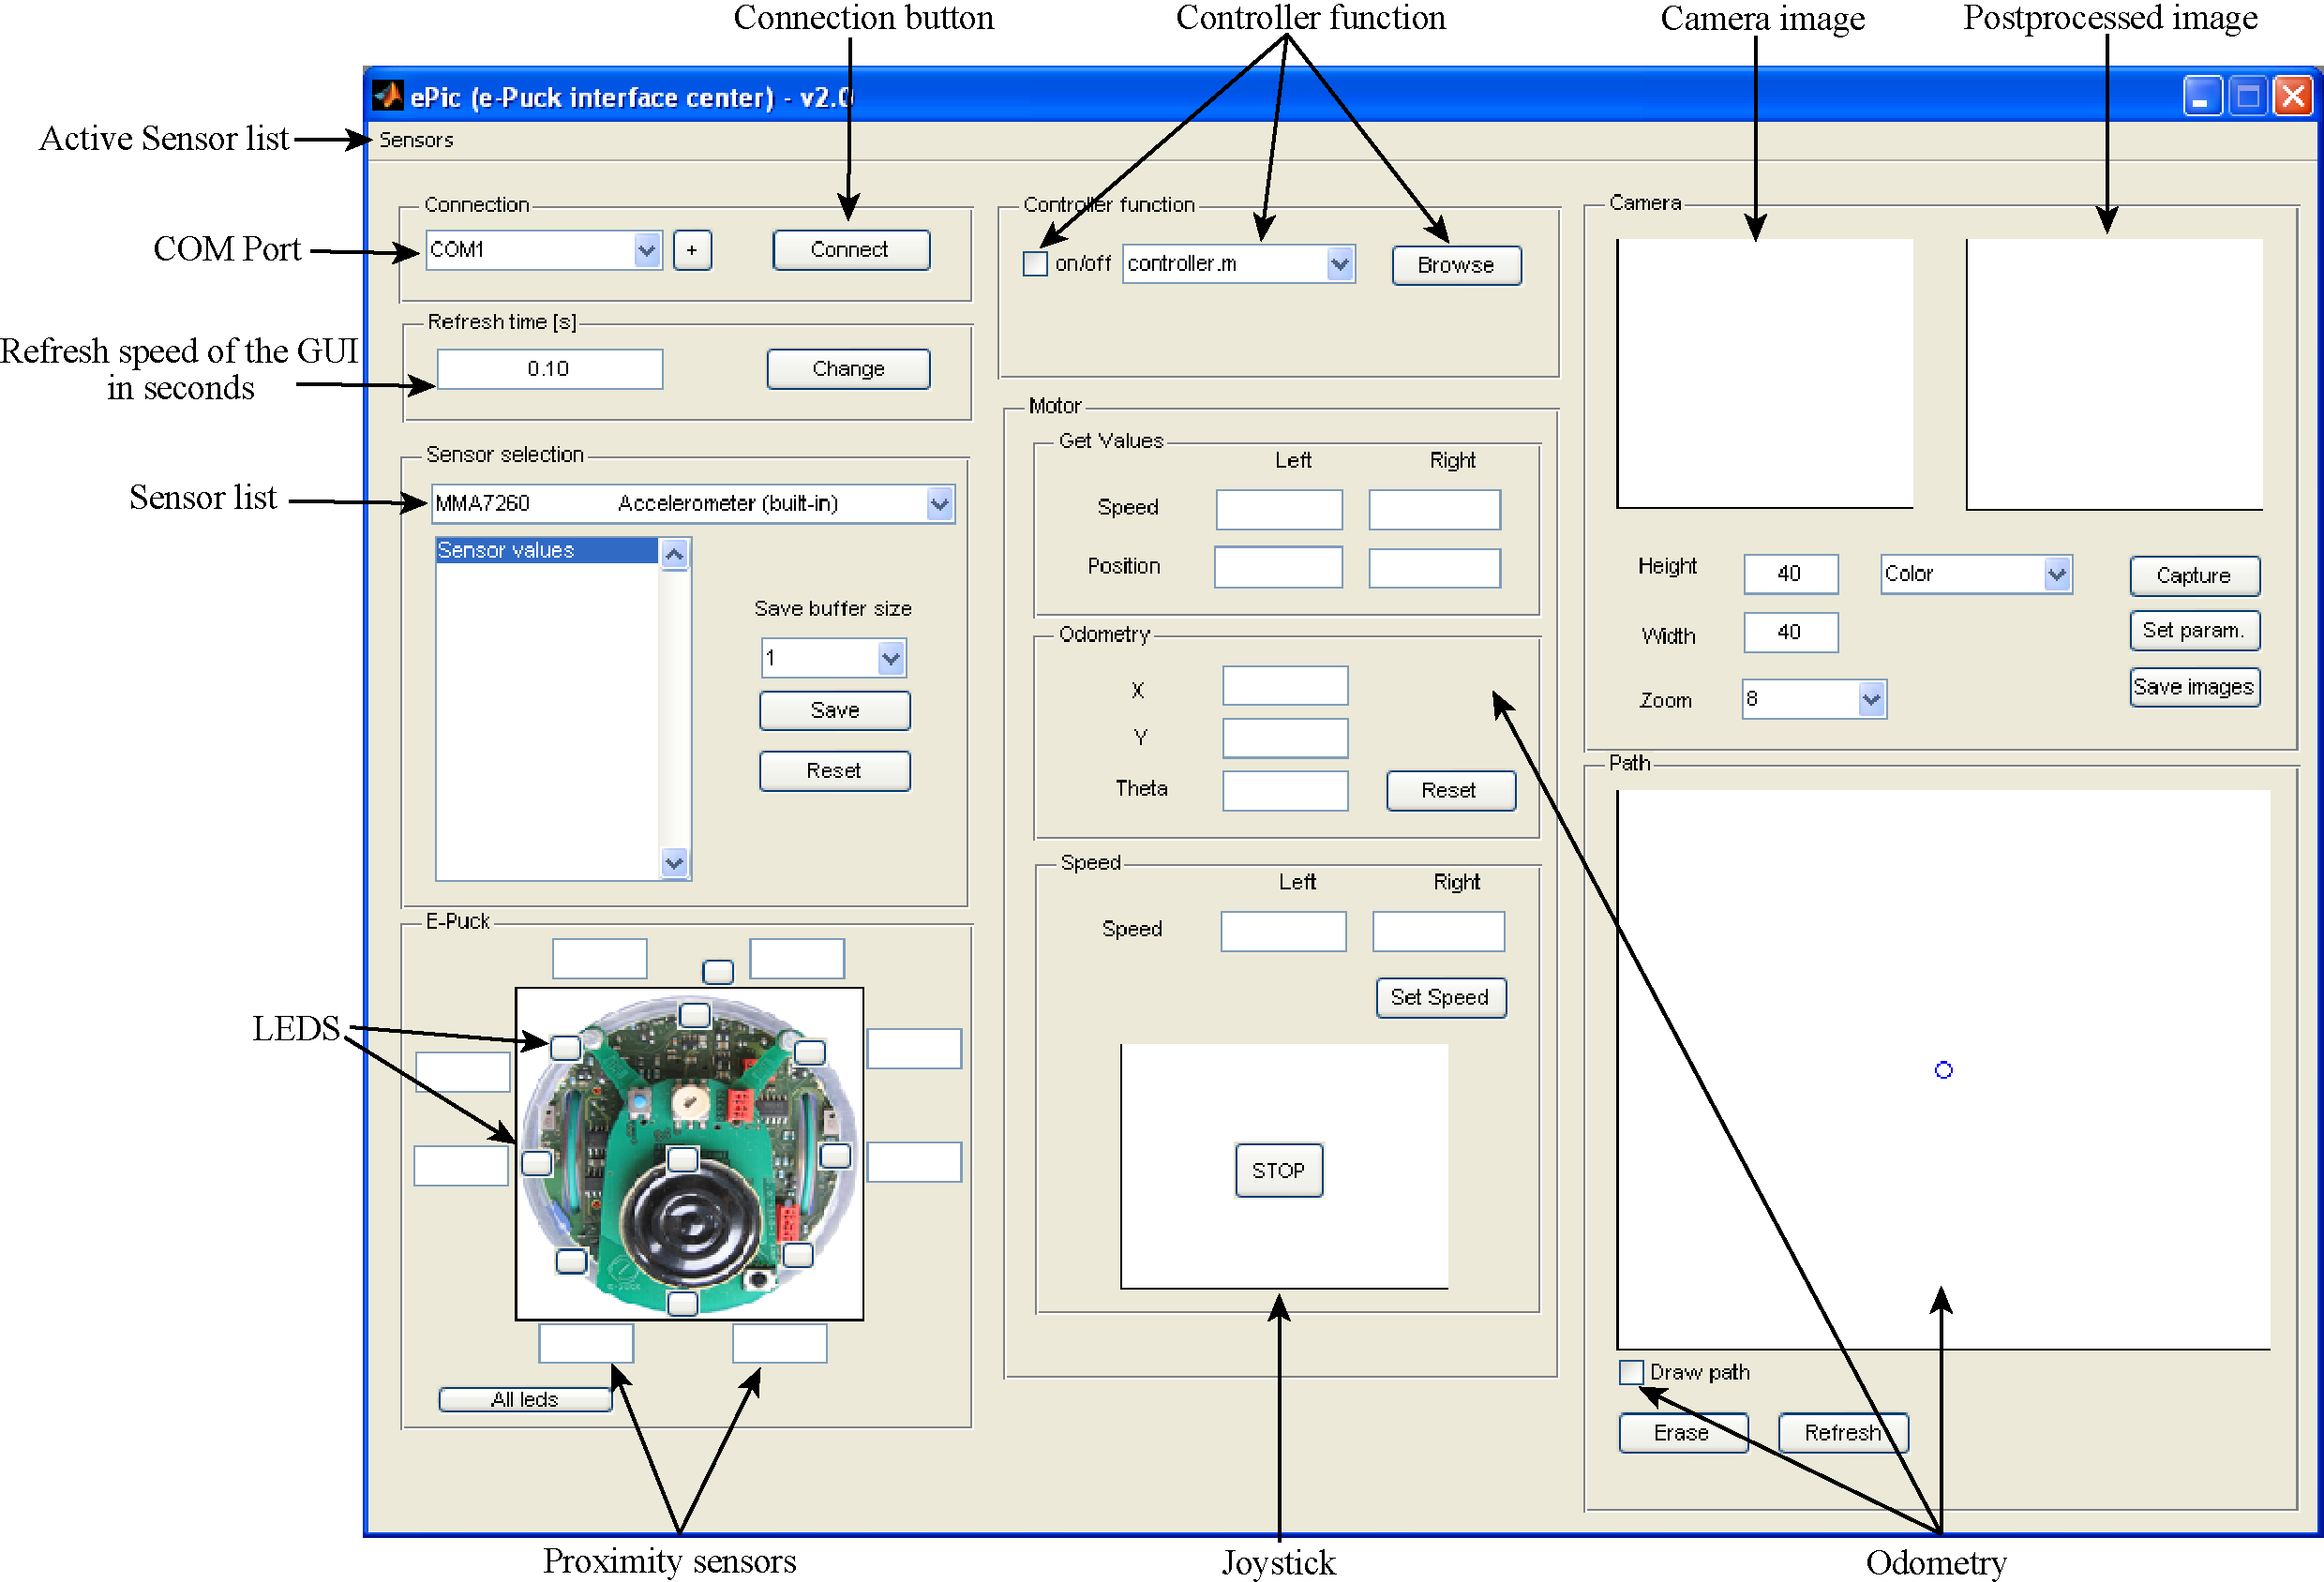
\includegraphics[width=1.10\textwidth]{ePic2.png}
	\caption{The ePic2 Graphical Interface\label{fig:epic}}
\end{figure}

\subsection{The Controller}
One feature of the GUI is the implementation of a controller function to command the e-puck. This function is located in the file \emph{controller.m} and is initially empty. Once activated, it can be programmed to add a behavior to the e-puck.
\par The controller acts as a Matlab script. As such, all the above functions can be used to command the e-puck. The command \emph{update} does not need to be called as it is done automatically by the interface. It is nevertheless necessary to activate the sensors you need for your controller before executing it.
\par The controller is a finite state machine. It begins in state 1 and executes its initialization. Then it moves to state 2 or more to execute the body of the code. When stopped, it goes to state -1 where it executes the final part of the code before going to state -2. If the controller crashes for no precise reason, the interface detects it and stops its execution.

\subsection{Sensor Captures}
The interface always saves the values of the currently selected sensor. A box allows to choose how many samples have to be kept. For instance, if 1 is selected, the last value will always be kept in memory. When you want to transfer the saved values to Matlab, press the button \emph{Save} and the last readings will be transfered to Matlab's workspace. In some cases, this button will be disabled and colored in red. It means that the minimum amount of samples requested has not been attained yet. When it will be so, the button will turn green. It is possible to save an undefined number of samples by choosing \emph{Unlimited} as Save buffer size.
\par The Reset button will empty the Save buffer. 

\subsection{Driving the Robot}
To drive the robot, you have two choices using the interface. You can either set a speed for each motor in the area \emph{Speed} and press the button \emph{Set Speed} or you can use the visual joystick underneath. The white zone of the joystick allows you to set the motor speeds using a more intuitive way. For instance, if you click the top middle of the white zone, the e-puck will run at maximum speed in straight direction. If you press a bit on the right, it will start to turn right. If you press below the button \emph{Stop} it will run backward. The \emph{Stop} button is used to stop the robot. 

\subsection{The Camera}
The camera area is composed of two displays. The first is the current view coming from the robot while the one on the right is the same view after filtering. The camera works in two modes: color or gray scale. The height and the width can be chosen but it should be carefully considered as the e-puck is quite limited in memory. The value 40x40 is an adequate value. The zoom factor describes a zoom out from the center of the image. By choosing 1, the image will be very neat but very focused while 8 gives a wider view with a reduced quality. The number that can be chosen are 1, 2, 4 and 8. After any modification of those values, the button \emph{Set param.} must be pressed to send them to the e-puck. When the button \emph{Capture} is pressed, a new snapshot is taken.

\section{Known issues}
The initial connection can take quite a long time sometimes. This is due to the Windows driver of some computers. Don't despair and wait. It will connect finally. When closing the connection, it is possible that Matlab crashes and has to be killed. This is also due to the Windows driver and occur only on some machines.

\section{Credits}
ePic2 was developed at the Laboratory of Intelligent Systems located in the Ecole Polytechnique F\'ed\'erale de Lausanne in Switzerland by Yannick Weibel and Julien Hubert.

\end{document}